\documentclass{article}
\usepackage{fullpage}
\usepackage{physics}
\usepackage{authblk}
\usepackage{indentfirst}
\usepackage{commath}
\usepackage{graphicx}
\usepackage{float}
\usepackage{subfig}
\usepackage{amsmath}
\usepackage{bm}
\usepackage[utf8]{inputenc}
\usepackage[T1]{fontenc}

\author{Hunter Belanger}

\title{Preliminary Analysis of Delta Tracking}
\date{}

\begin{document}
	\maketitle
	
	\section{Description of System}
	 The system which I have chosen to build this toy model around is a slab reactor, which is infinite in two dimensions, and finite along the x axis, with vacuum at either end of the reactor. The reactor itself is composed of a core which is a multiplying medium, and a reflector at either side which is non-multiplying. A depiction of this system along the x axis is presented below in Figure~\ref{fig:réacteur}.
	
	\begin{figure}
		\centering
		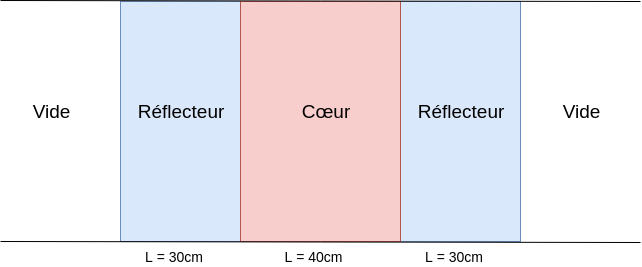
\includegraphics[scale=0.45]{reacteur.png}
		\caption{Reflected slab reactor, finite in x axis, infinite in y and z.}
		\label{fig:réacteur}
	\end{figure}
	
	The two group approximation is used in these programs, with the assumption of isotropic scattering for the moment. the cross sections for each material at each energy are provided in tables bellow (with scattering matrices).
	
	\begin{table}
		\centering
		\begin{tabular}{|c|c|c|}
			\hline
			\textbf{Cross Section} & \textbf{Reflector} & \textbf{Core} \\ 
			\hline \hline
			$\Sigma_{t_1}$ & 0.295 & 0.276 \\
			$\Sigma_{t_2}$ & 2.1 & 1.063 \\
			\hline
			$\Sigma_{a_1}$ & 0.0004 & 0.012 \\
			$\Sigma_{a_2}$ & 0.02 & 0.121 \\
			\hline
			$\Sigma_{f_1}$ & 0.0 & 0.00339 \\
			$\Sigma_{f_2}$ & 0.0 & 0.074 \\
			\hline
			$\nu_1$ & 0.0 & 2.5 \\
			$\nu_2$ & 0.0 & 2.5 \\
			\hline
		\end{tabular}
		\caption{Cross sections for the system (in units of $cm^{-1}$), except scattering matrices.}
	\end{table}
	
	\begin{table}
		\centering
		\subfloat[Reflector]{
			\begin{tabular}{|c | c | c |}
				\hline
				 & \textbf{to 1} & \textbf{to 2} \\
				 \hline
				 \textbf{1} & 0.2456 & 0.049 \\
				 \hline
				 \textbf{2} & 0.0 & 2.08 \\
				 \hline				
			\end{tabular}
		}
		\hspace{50pt}
		\subfloat[Core]{
			\begin{tabular}{|c | c | c |}
				\hline
				& \textbf{to 1} & \textbf{to 2} \\
				\hline
				\textbf{1} & 0.25 & 0.014 \\
				\hline
				\textbf{2} & 0.0 & 0.942 \\
				\hline				
			\end{tabular}
		}
		\caption{Scattering matrices, $\Sigma_{j\rightarrow i}$, for the system (in units of $cm^{-1}$).}
	\end{table}
	
		\subsection{Baseline Solution}
		Two solutions for the eigenvalue of this system were obtained using MCNP and OpenMC. MCNP was also used to calculate the scalar flux for each neutron group. These calculations were done with 1000000 histories, at 1015 generations (15 of which were ignored).
		
		\begin{table}
			\centering
			\begin{tabular}{|c|c|}
				\hline
				\textbf{Platform} & \bm{$k_{eff}$} \\
				\hline
				\hline
				MCNP & 1.00914 $\pm$ 0.00002 \\
				\hline
				OpenMC & 1.00915 $\pm$ 0.00002 \\
				\hline
			\end{tabular}
			\caption{Criticality of the system.}
			\label{tab:crit}
		\end{table}
		
		The criticity from MCNP in Table~\ref{tab:crit} shall be considered the true eigenvalue for this system for the purposes of this work. The normalized scalar flux from MCNP (with error bars) is presented in Figure~\ref{fig:mcnp_flux}. The error of the scalar flux is plotted for reference in Figure~\ref{fig:mcnp_flux_erreur}.
		
		\begin{figure}
			\centering
			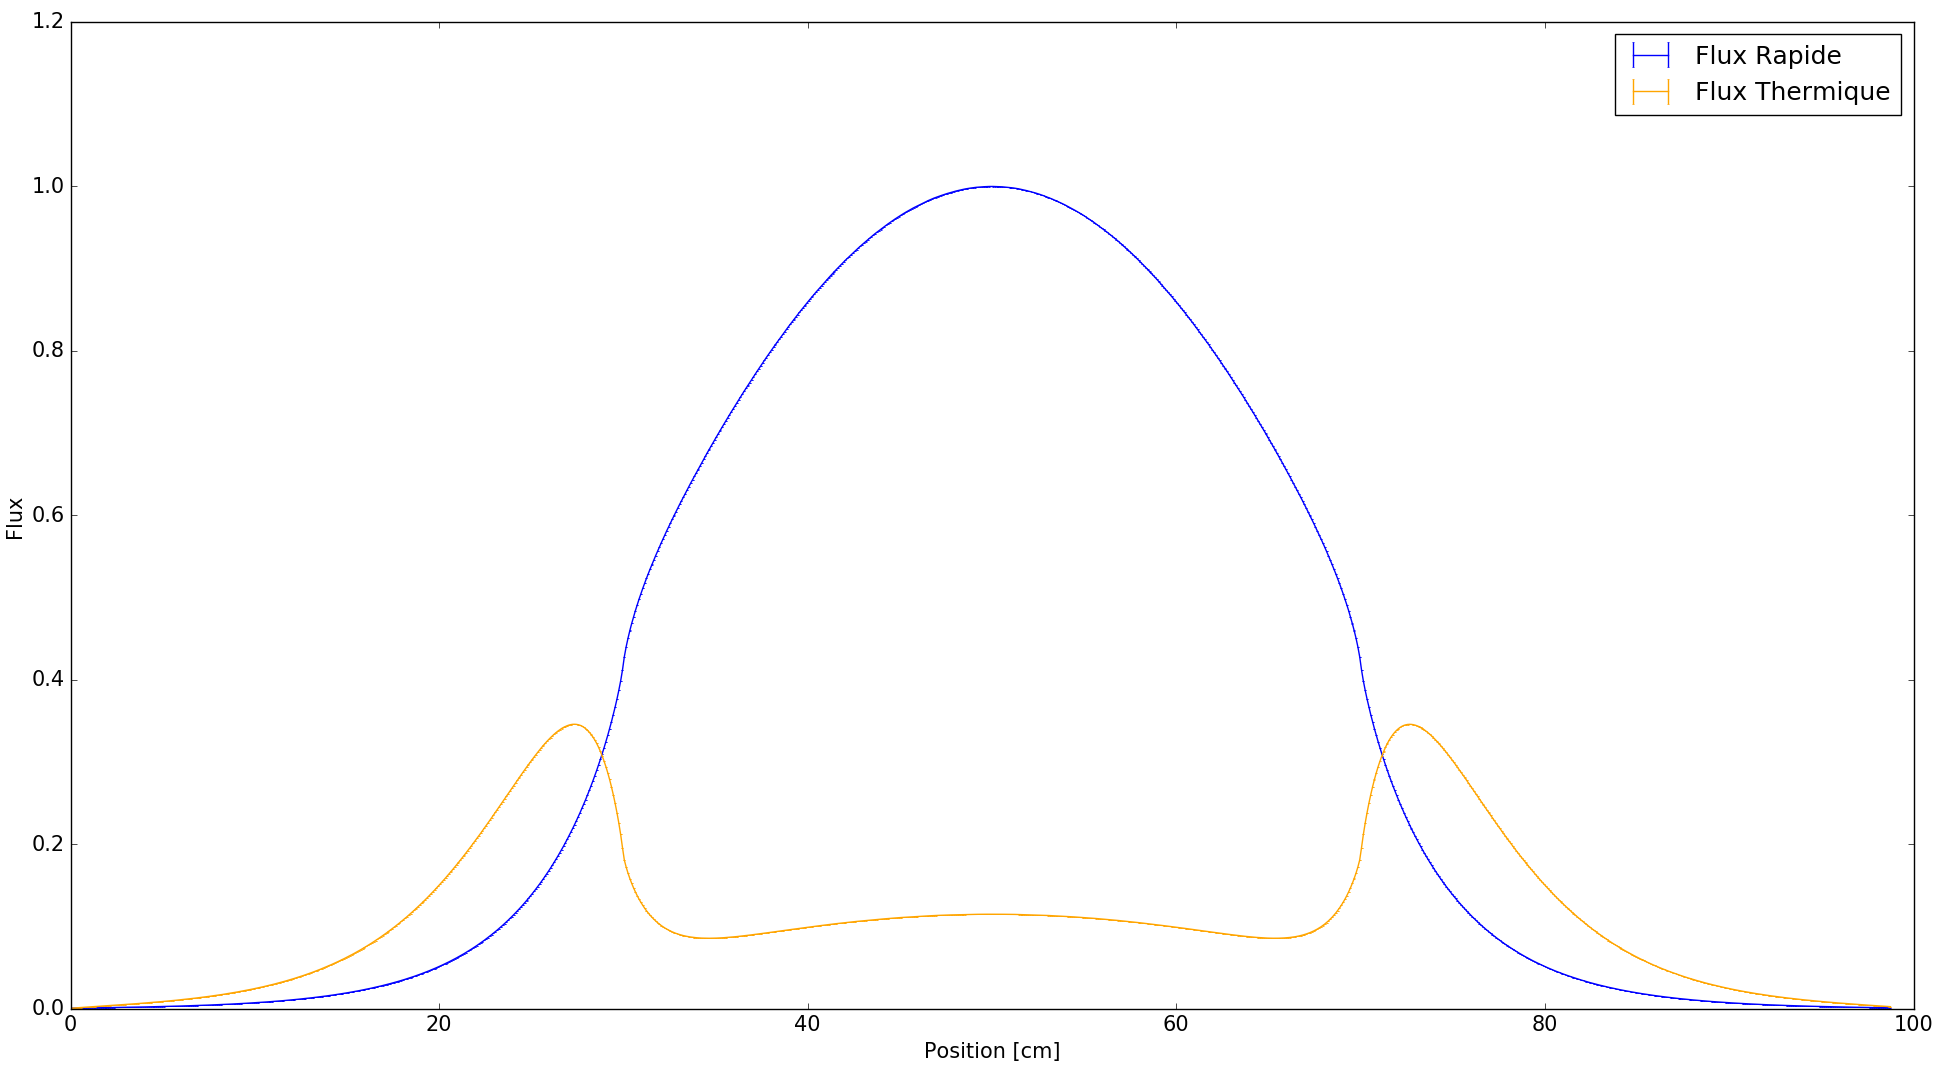
\includegraphics[scale=0.35]{mcnp_flux.png}
			\caption{MCNP scalar flux with error bars.}
			\label{fig:mcnp_flux}
		\end{figure}
	
		\begin{figure}
			\centering
			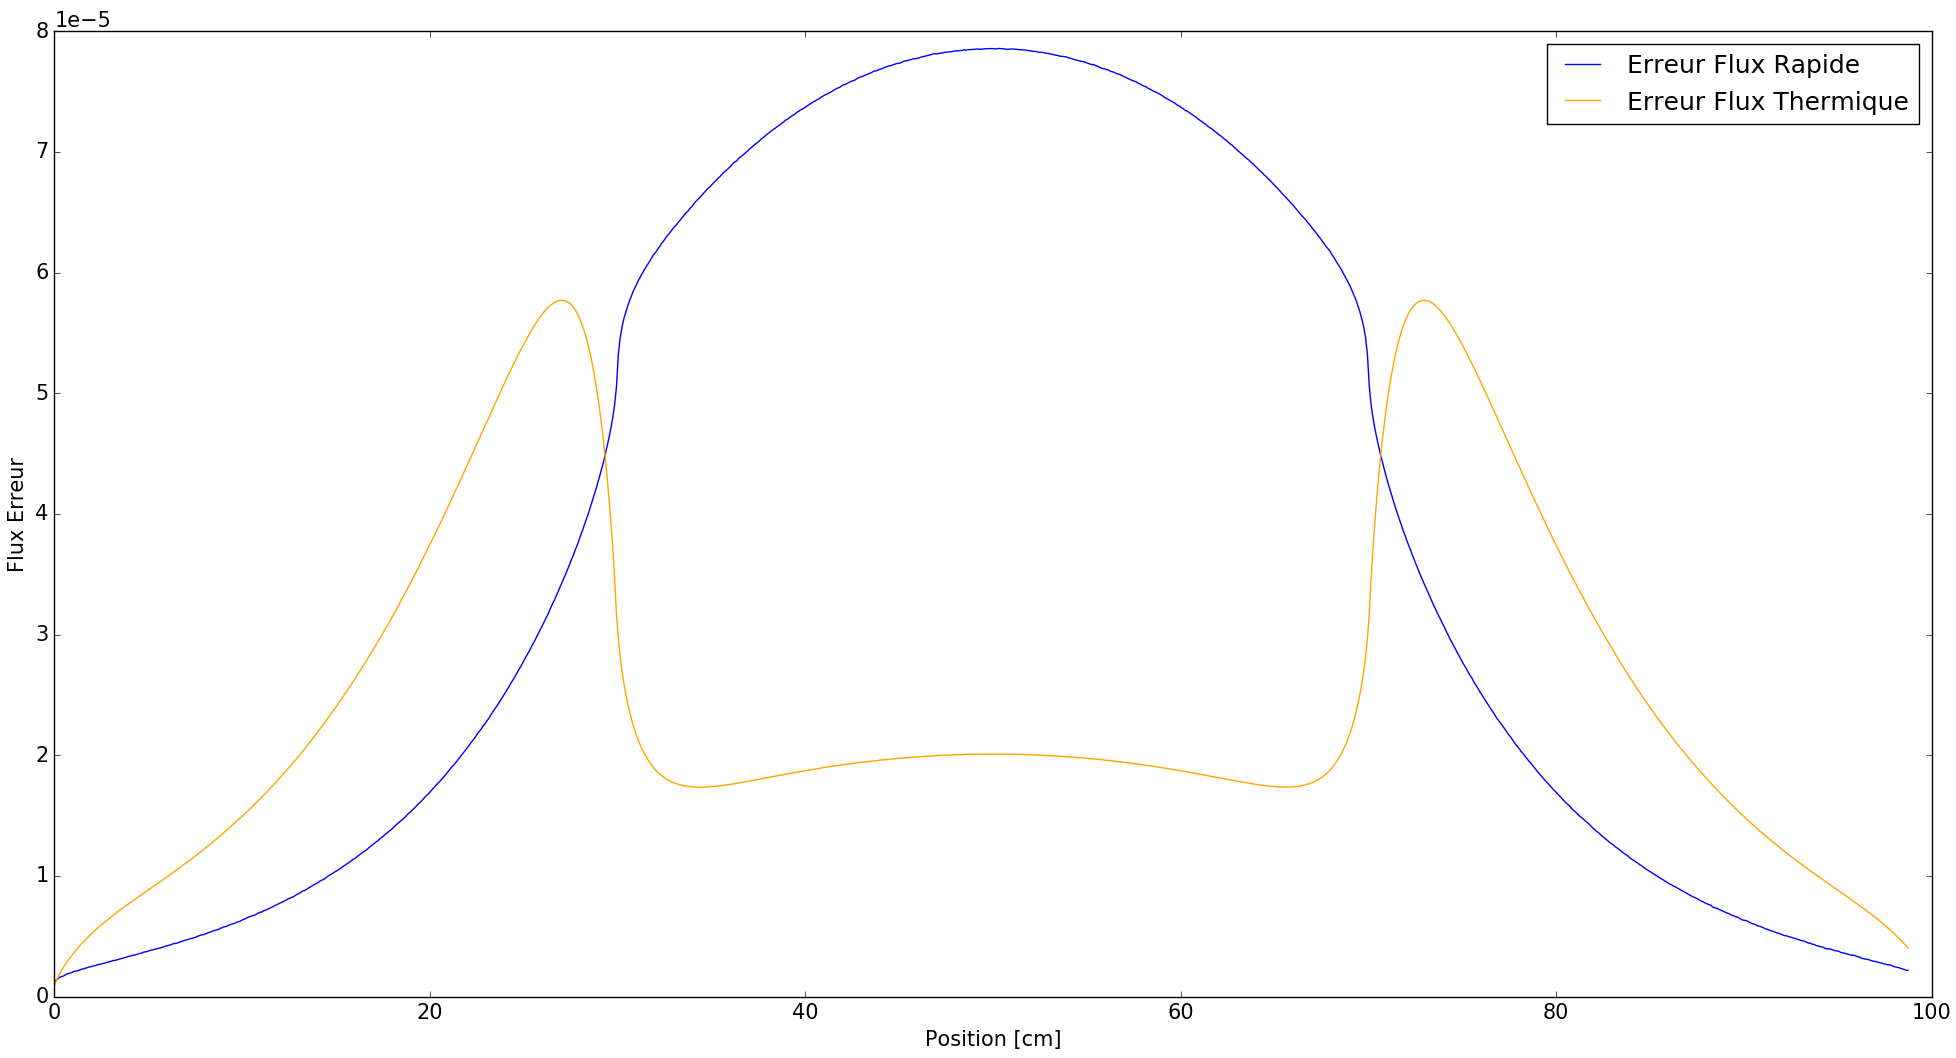
\includegraphics[scale=0.35]{mcnp_flux_erreur.png}
			\caption{MCNP scalar flux error.}
			\label{fig:mcnp_flux_erreur}
		\end{figure}
	
		\subsection{Calculation Methods}
			Here are outlined the methods used to make the calculations of the flux, entropy, and FOM. The following codes all use the same methods to calculate these values to minimize differences between results that are not directly related to the tracking method (ray-tracing, delta-tracking, etc.).
			\subsubsection{Scalar Flux}
			To calculate the scalar flux, the core was divided into 1000 bins along its x axis, each with a thickness of 0.1$cm$. Each time a neutron underwent a collision, the flux tally in that bin was increased with: 
			\begin{equation}
				F_{E,b} \quad += \quad \frac{w}{\Sigma_t(x)}
			\end{equation}
			where $F_{E,b}$ is the flux tally in bin $b$ for energy group $E$. Bin $b$ corresponds to the location of the collision ($x$), and $w$ is the weight of the neutron. It is not necessary to normalize the box by size as all boxes have the same size, and only the normalized scalar flux is being considered. 
			
			\subsubsection{Entropy}
			In a similar manner to the flux, the entropy was calculated for each generation, with the core region being divided into 200 bins, with a thickness of 0.2$cm$. The number of neutrons in box $b$ at the beginning of the generation is $N_b$, and the value of the entropy for the generation is calculated as
			\begin{equation}
				H = \sum_{b} N_b \log_2(N_b)
			\end{equation}
			where it is assumed all boxes have at least 1 neutron. This is a valid assumption for these cases with large bins and a large number of histories per generations.
			
			\subsubsection{Figure of Merit}
			The Figure of Merit (FOM) is calculated with the following formula:
			\begin{equation}
				FOM = \frac{1}{T\big(\frac{\sigma}{k_{avg}}\big)^2}
			\end{equation}
			where $T$ is the time in seconds since the first generation which was not ignored began, and $\sigma$ is the standard deviation of the current average for the criticality of the system, $k_{avg}$.
			
	\subsection{Russian Roulette}
	As the neutrons are weighted, Russian roulette is played to kill particles who become "unimportant" due to their low weight. This is done with a cutoff weight of $0.25$ and a survival weight of $1.0$.
	
	\section{Ray Tracing Program}
	The ray-tracing model is found in the "ray\_trace" directory. This program was written first, and uses what I believe to be a standard ray-tracing method. The flight distance is calculated with
	\begin{equation}
		d = -\frac{\ln(\xi)}{\Sigma_T}.
	\end{equation}
	The distance to the nearest surface is then calculated based on the particles flight direction, and a comparison is made: If the distance $d$ is shorter than the distance to the closest surface ($d_{surf}$) then the particle is moved by a distance $d$ and of course stays within the same cell and material. Should the converse be the case, the particle is moved a distance $d_{surf} + \epsilon$ so that it is just on the other side of the surface, and is in the new material. A new travel distance is then calculated as before with the new cross section.
	
	This program came up with an eigenvalue of $k_{eff} = 1.00908 \pm 0.00002$. The plot of the flux and flux error and provided in Figures~\ref{fig:rt_flux} and \ref{fig::rt_flux_erreur} respectively.The full simulation output is found in the ray\_trace directory, in the text file terminal\_output.
	
	
	\begin{figure}
		\centering
		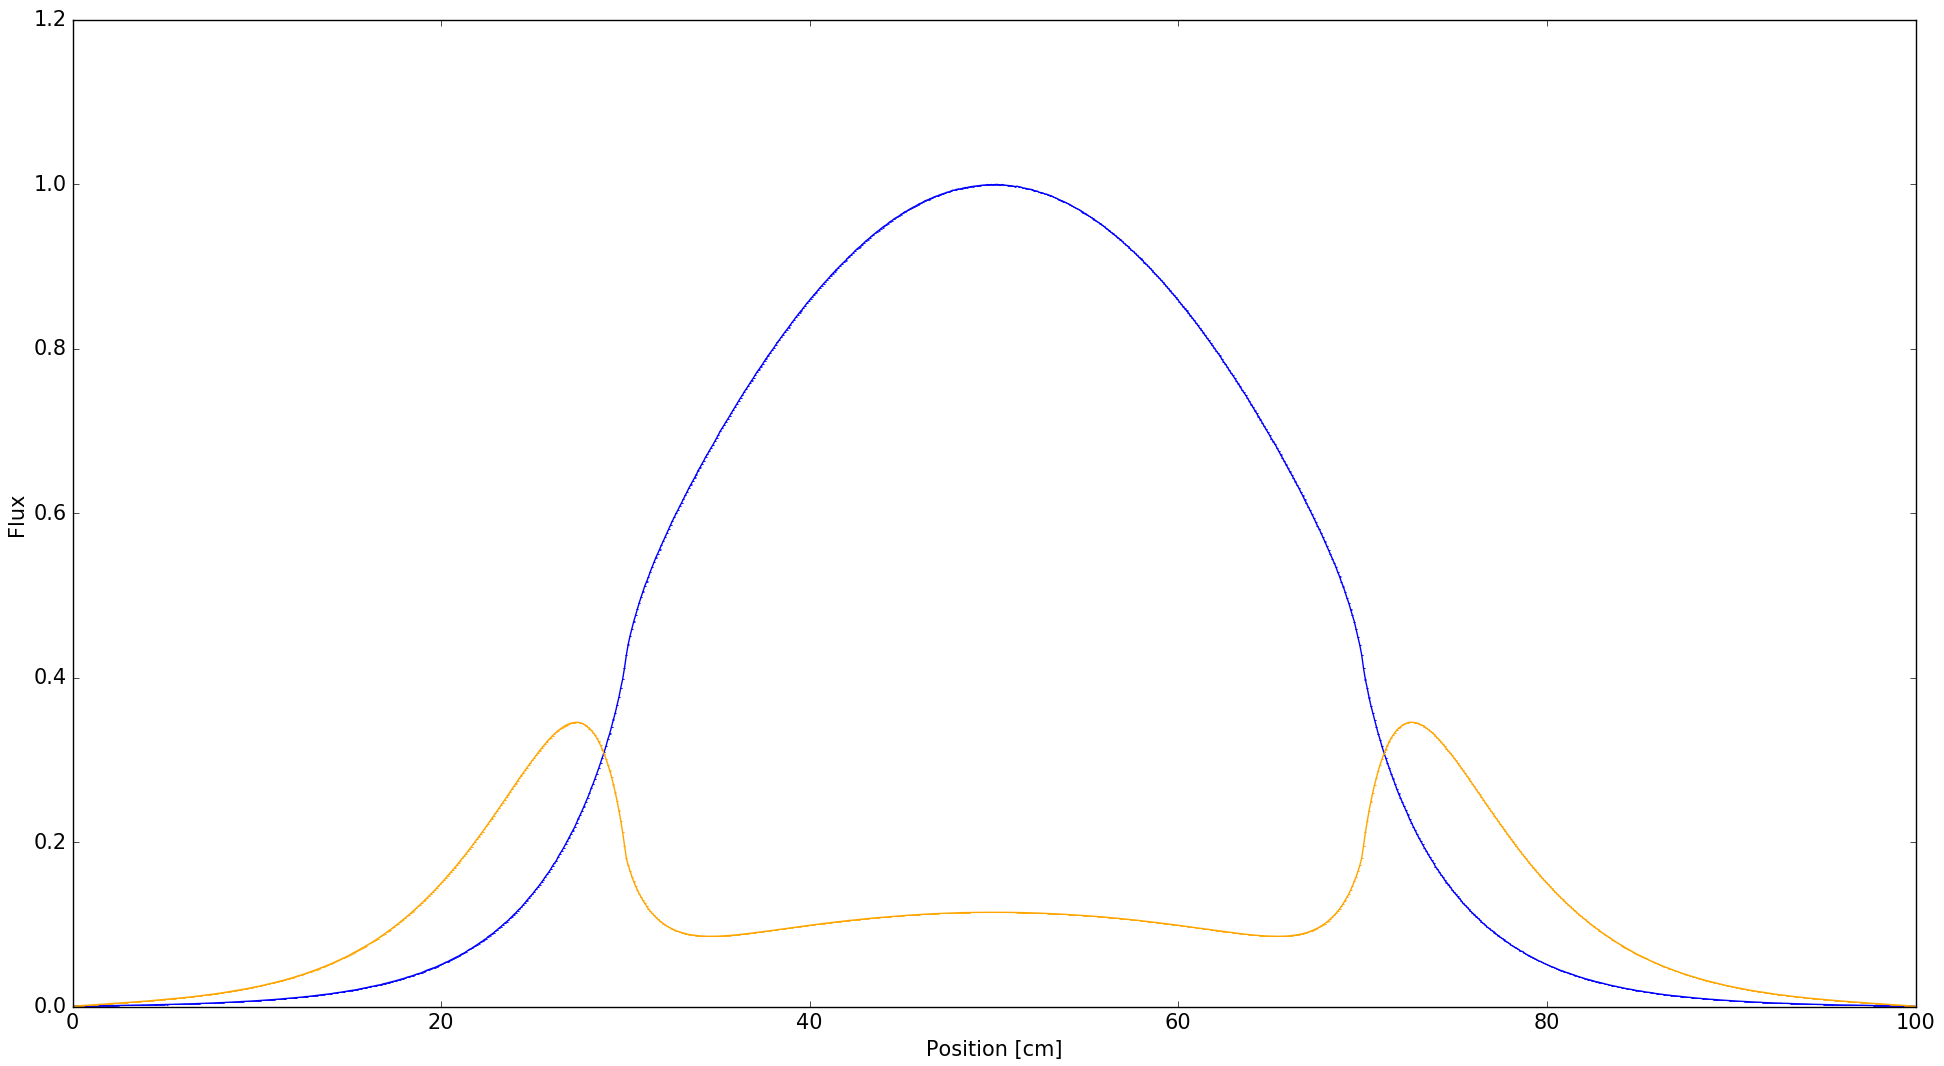
\includegraphics[scale=0.35]{rt_flux.png}
		\caption{Ray-tracing flux with error bars.}
		\label{fig:rt_flux}
	\end{figure}
	\begin{figure}
		\centering
		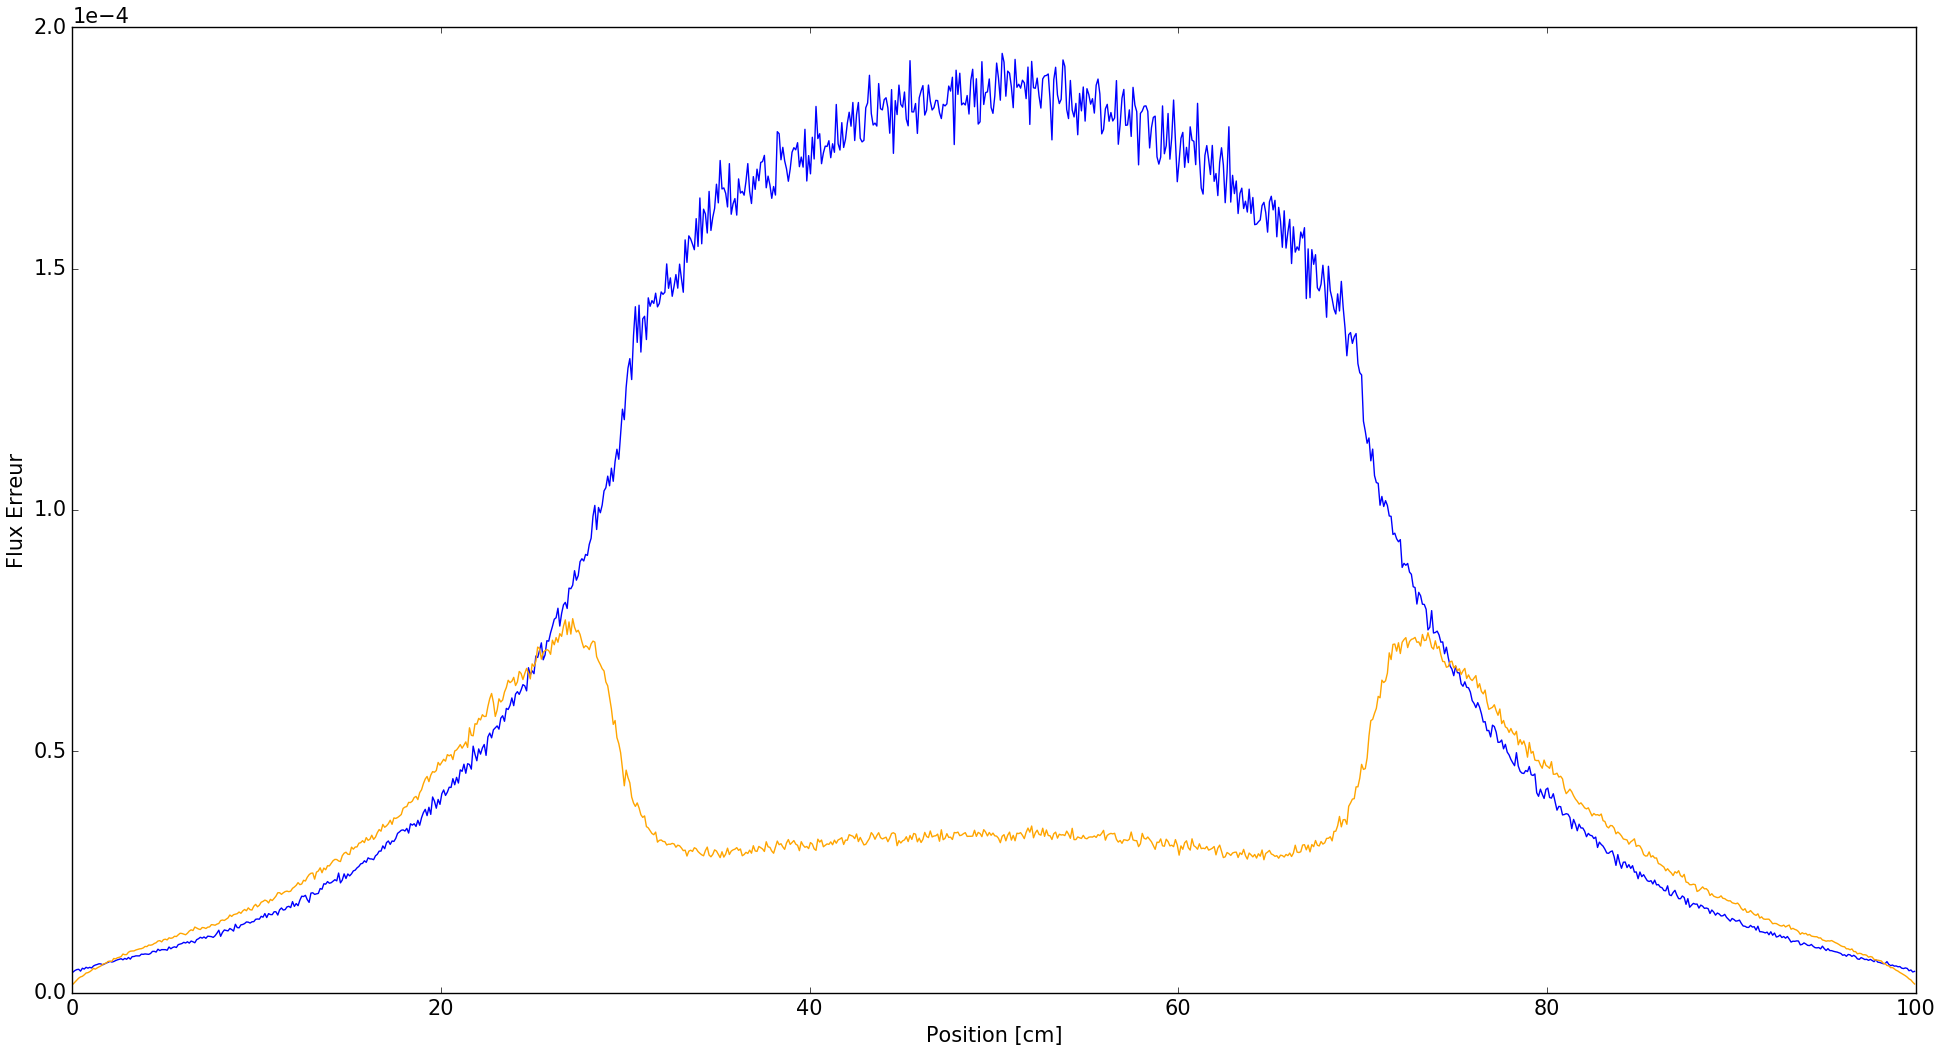
\includegraphics[scale=0.35]{rt_flux_erreur.png}
		\caption{Ray-tracing flux error.}
		\label{fig::rt_flux_erreur}
	\end{figure}
	
	\section{Delta Tracking Program}
	Delta tracking works in a slightly different way than ray-tracing. Instead of making a check to see if the distance to the surface of a cell is shorter than the sampled flight distance, a flight distance which is valid for the entire system is calculated, replacing the material cross section $\Sigma_T$ with the majorant cross section for the system $\Sigma_M$. The particle is then moved that distance, and its current location and material are sampled. Using the actual cross section at the particle location $\Sigma_T(x)$, if
	\begin{equation}
		\xi < \frac{\Sigma_T(x)}{\Sigma_M}, \quad \xi \in [0,1)
		\label{eq:virtual_col}
	\end{equation}
	the collision is accepted as being real. Otherwise a virtual collision has occurred. Should this be the case, the particle may then be "kicked" forward an additional distance by calculating a new distance as before. The second option, labeled no\_kicking in the delta\_tracking directory, simply moves the particle back to it's original location, and samples a new flight distance.
	
	\subsection{Particle Escape}
	Basic delta-tracking as described in papers has one minor oversight, and that is how to deal with particles escaping to a vacuum region. With ray-tracing, it's quite simple: the particle is moved just barley into the vacuum region when it crosses the cell boundary, and it finds that $\Sigma_T=0$, causing it to have an infinite flight distance and escapes.
	
	Delta tracking does not keep track of when a particle crosses a surface boundary. As such, a particle may cross into vacuum, and a virtual collision check will occur. At this point, the probability of a virtual collision is now exactly zero due to Equation~\ref{eq:virtual_col}. With no change in particle energy or direction, an infinite loop occurs where a collision may never be accepted.
	
	To get around this dilemma, I wrote the program so that if a particle does find itself in a vacuum, it is considered dead and no check for a virtual or real collision is made. This should be a valid assumption to make as it is possible and valid to switch from delta-tracking to ray-tracing for different flights.
	
	\subsection{Results}
	As it turns out, the "kicking" method and "no\_kicking" method of delta tracking are equivalent models, due to the exponential functions being memoryless. As such, only the eigenvalue and flux plots for the kicking version of the model are shown. The determined eigenvalue was $k_{eff} = 1/00914 \pm 0.00002$. The flux and flux error are shown in Figures~\ref{fig:dt_flux} and \ref{fig:dt_flux_error}.
	
	\begin{figure}
		\centering
		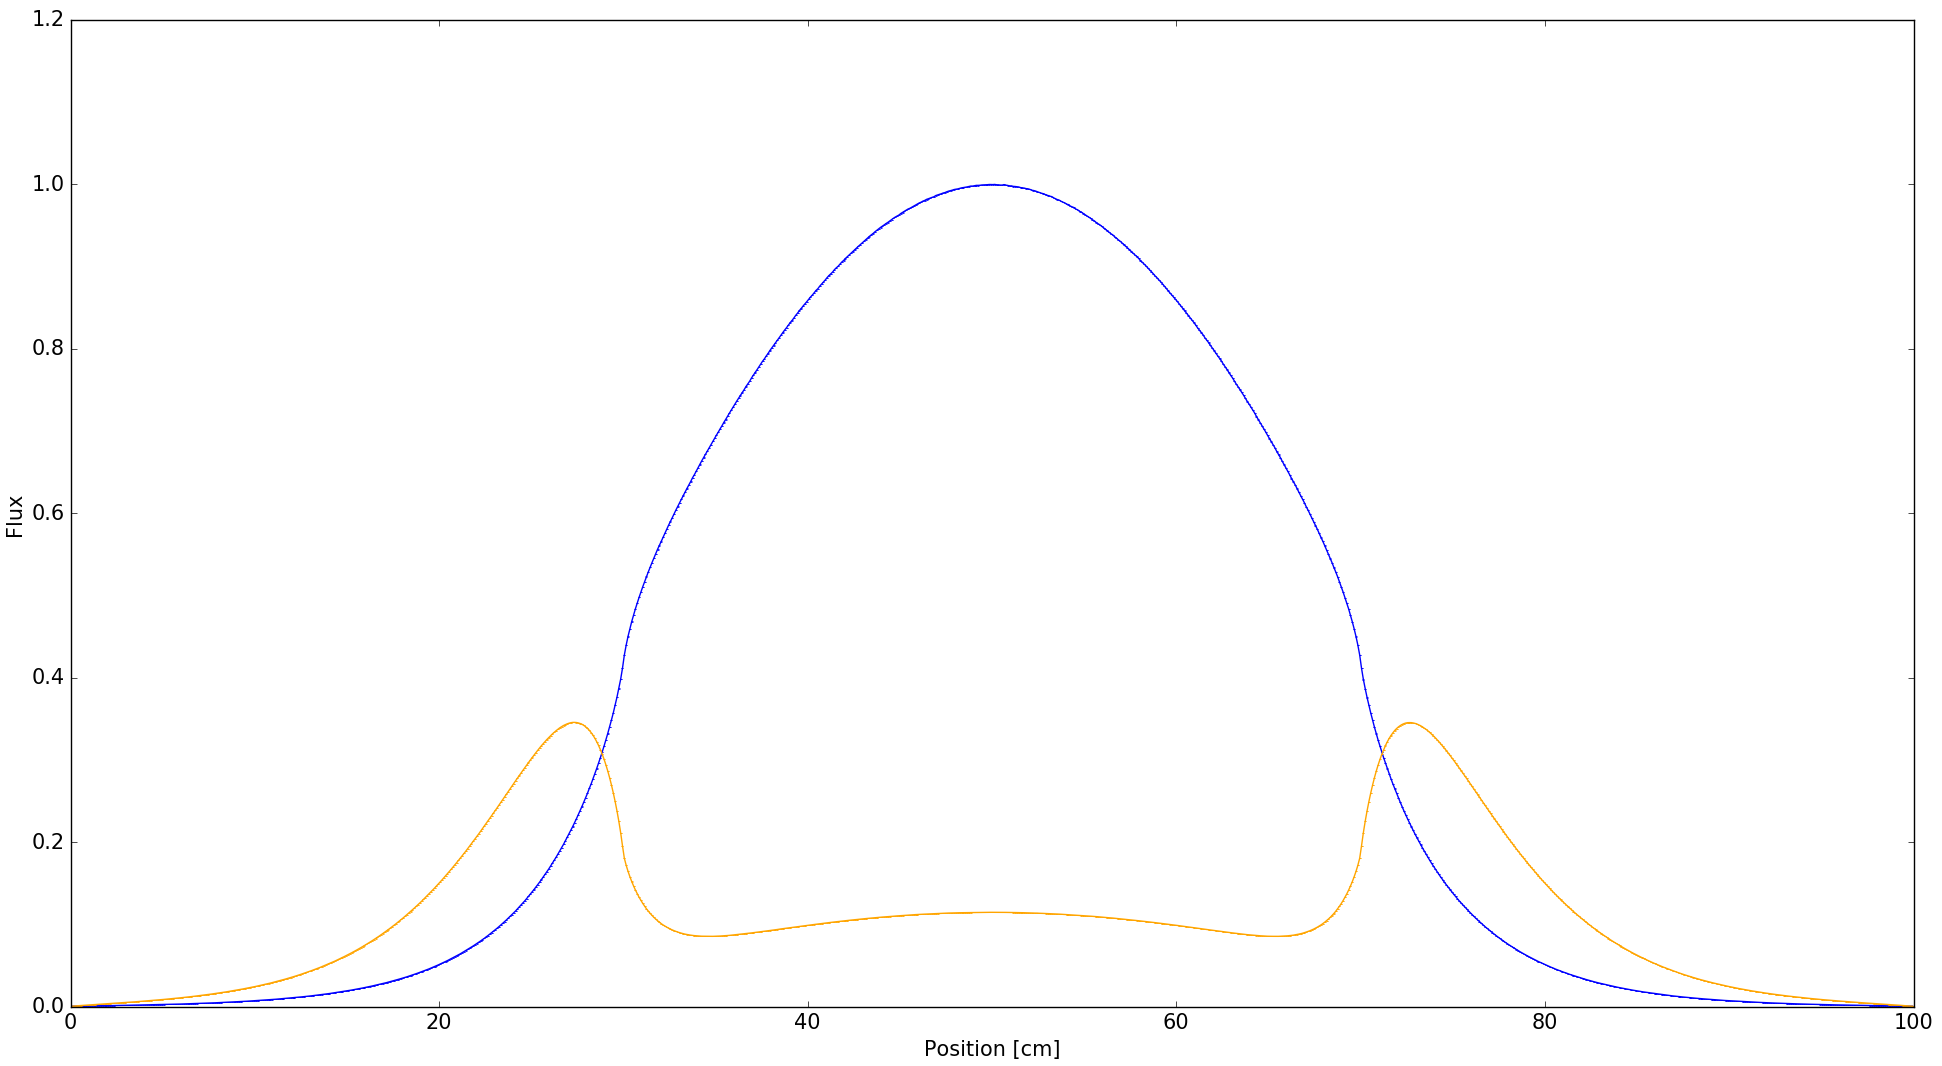
\includegraphics[scale=0.35]{dt_flux.png}
		\caption{Delta-tracking scalar flux with error bars.}
		\label{fig:dt_flux}
	\end{figure}
	\begin{figure}
		\centering
		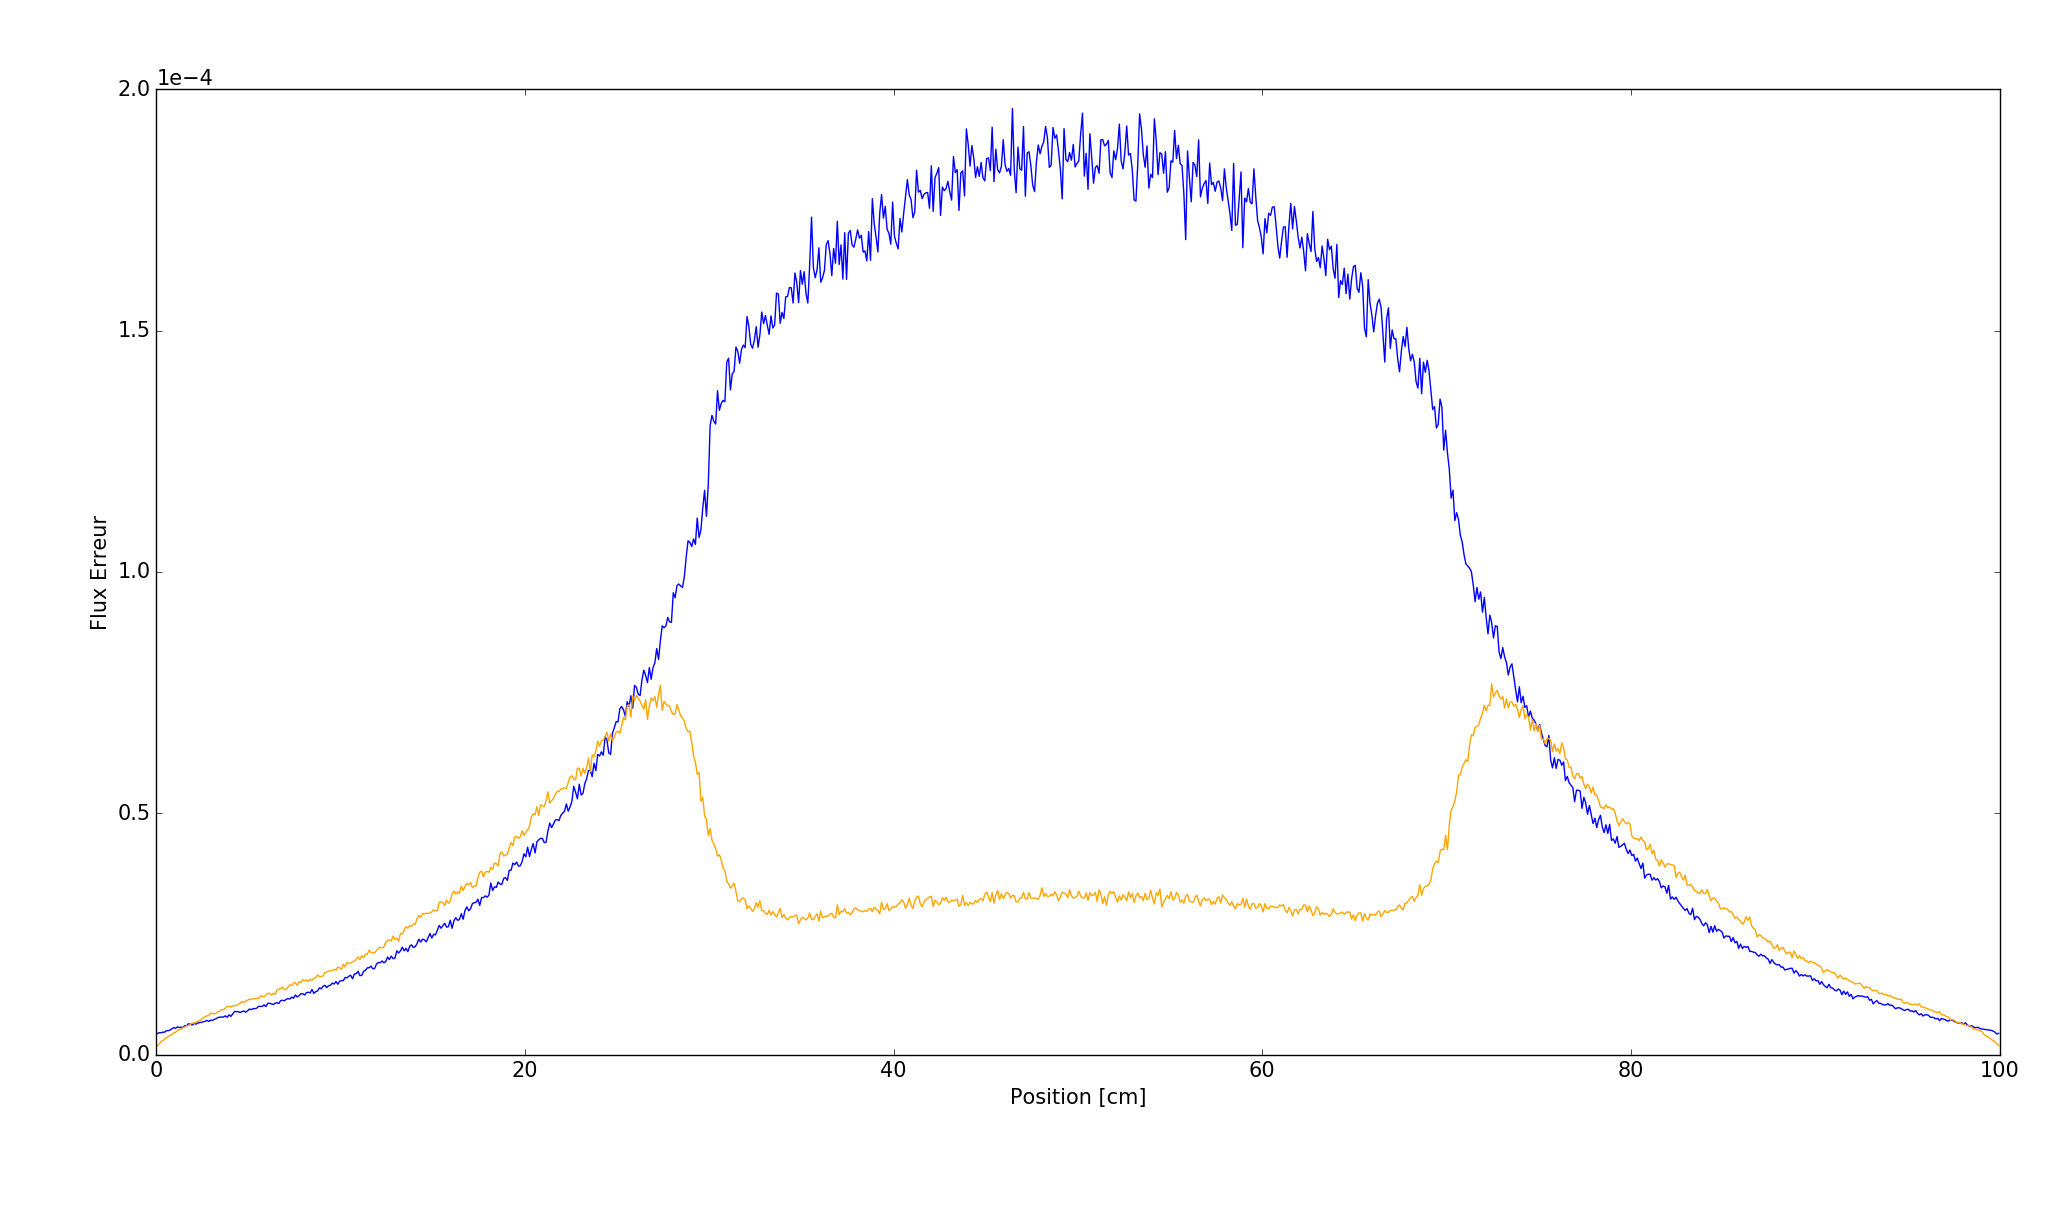
\includegraphics[scale=0.3]{dt_flux_erreur.png}
		\caption{Delta-tracking scalar flux error.}
		\label{fig:dt_flux_error}
	\end{figure}
	
\end{document}